\begin{minipage}[t]{.35\textwidth}%
%\large



\textbf{Flüssigkeiten \& Gase}\par \vspace*{-4mm}
%\begin{spacing}{1.5}
\begin{align*}
&\text{Druck:} ~ p = \frac{F}{A} \\
&\text{Kontinuitätsgleichung:} ~ A_1 \cdot v_1 = A_2 \cdot v_2 \\
&\text{Bernoulli:} 		~ p + \rho g h + \frac{1}{2} \rho v^2 = \text{const.} \\[-4pt]
&\quad \text{Staudruck (nach Bernoulli):} ~ p = \frac{1}{2} \rho v^2 \\[-4pt]
&\quad \text{Druck in Wassersäule:} ~ p = \rho gh \\
&\text{Toricelli (Ausfließgeschw.)}: ~ v = \sqrt{2gh} \\[-2pt]
&\qquad t = \sqrt{\frac{2}{g}} \cdot \frac{A_1}{A_2} \cdot (\sqrt{h_{\alpha}}-\sqrt{h_{\omega}})
\end{align*}

\vspace*{8mm}
\textbf{Strömung mit Reibung}\par \vspace*{-4mm}
\begin{align*}
&\text{Volumenstrom:}	~ \dot{V} = \frac{V}{t} = A \cdot \overline{v}\\
&\text{Schubspannung:}	~ \tau = \eta \cdot \frac{d v}{d z} = \frac{F_{R}}{A} \\
&\text{Viskosität:}	~ \eta = \frac{\tau}{D} \\
&\text{Hagen - Poiseuille:} ~ \dot{V} = \frac{\pi R^4}{8\eta} \cdot \frac{d p}{d x}\\
&\text{Leistung} ~ P = \frac{8\eta \cdot \Delta l}{\pi \cdot R^4} \cdot \dot{V}^2\\
&\text{mittlere}\\[-10pt] &\text{Strömungsgeschwindigk.:} ~  c = \overline{v} = \frac{1}{2} \cdot v_{max}
\\ \\
&\text{Stokes'sches Gesetz:} ~ F_r = 6 \pi \eta v r \\[-4pt]
&\quad \text{Stat. Sinkgeschwindigk.:} ~ v = \frac{2r^2g(\rho_1-\rho_2)}{9\eta} \\ \\
&\text{Gesamtwiderstand:} ~ F_{tot} = F_r + F_w\\[-4pt]
&\quad \text{Reibungswiderstand:}  ~ F_r = \eta \cdot A \cdot \frac{d v}{d z}\\[-2pt]
&\quad \text{Widerstandskraft:}  ~ F_w = c_w \cdot A \cdot \frac{1}{2} \rho v^2 \\
\\ 
\end{align*}
\textbf{Rheologie }\par 
\begin{tikzpicture}
\node(a)at(0,0){
\begin{tikzpicture}
\node[align=center,scale=0.8](1)at(0.5,1.5){Newtonsch};
\draw (0,1)node[right]{$\tau$} -- (0,0) -- (1,0)node[right,scale=0.8]{$D$};
\draw[yshift=-1.5cm] (0,1)node[right]{$\eta$} -- (0,0) -- (1,0)node[right,scale=0.8]{$D$};
\draw[black!80] (0,0) -- (0.9,0.9);
\draw[black!80,yshift=-1.5cm] (0,0.5) -- (0.9,0.5);
\end{tikzpicture}
};
\node(b)at(2,0){
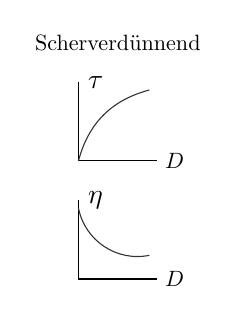
\begin{tikzpicture}
\node[align=center,scale=0.8](1)at(0.5,1.5){Scherverdünnend};
\draw (0,1)node[right]{$\tau$} -- (0,0) -- (1,0)node[right,scale=0.8]{$D$};
\draw[yshift=-1.5cm] (0,1)node[right]{$\eta$} -- (0,0) -- (1,0)node[right,scale=0.8]{$D$};
\draw[black!80] (0,0) to [bend left=30] (0.9,0.9);
\draw[black!80,yshift=-1.5cm] (0,0.9) to [bend right=45] (0.9,0.3);
\end{tikzpicture}
};
\node(c)at(4.5,0){
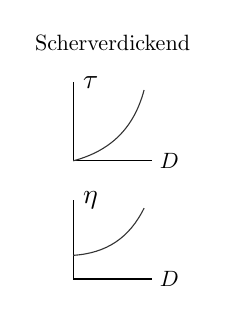
\begin{tikzpicture}
\node[align=center,scale=0.8](1)at(0.5,1.5){Scherverdickend};
\draw (0,1)node[right]{$\tau$} -- (0,0) -- (1,0)node[right,scale=0.8]{$D$};
\draw[yshift=-1.5cm] (0,1)node[right]{$\eta$} -- (0,0) -- (1,0)node[right,scale=0.8]{$D$};
\draw[black!80] (0,0) to [bend right=30] (0.9,0.9);
\draw[black!80,yshift=-1.5cm] (0,0.3) to [bend right=30] (0.9,0.9);
\end{tikzpicture}
};
\node[scale=0.7,rotate=90](fl)at(-1,0.55){Fließkurve};
\node[scale=0.7,rotate=90,align=left](vi)at(-1,-1){Viskositäts-\\kurve};
\end{tikzpicture}
%\end{spacing}
\vfill
\end{minipage}%
%\hspace*{2mm}
%\color{gray!40}
%\vrule
%\color{black}
\hfill
\begin{minipage}[t]{.35\textwidth}
%\large

\textbf{Einheiten \& Konstanten}\par \vspace*{-4mm}

\begin{align*}
%\text{Joule [J]} ~ 	= \frac{\kg \cdot \m^2}{\s^2} \\ %AUSGEBLENDET
&\text{Newton [N]} ~	= \frac{\kg \cdot \m}{\s^2} \\
&\text{Pascal [Pa]} ~	= \frac{\kg}{\m \cdot \s^2} = \ddfrac{\text{N}}{\m^2} \\ 
&\text{Viskosität [$\eta$]} ~	= \text{Pa}\cdot \s = \frac{\text{N} \cdot \s}{\m^2} \\ 
&\text{Watt [W]} ~ = \frac{\kg \cdot \m^2}{\s^3} = \frac{J}{s}\\ \\
&\text{Kritische Reynoldszahl:} \quad \text{Re}_{\text{krit}} = \frac{\rho d v}{\eta} = 2300 \\[-4pt] 
&\text{Stefan-Boltzmann Konst.:} ~\sigma = 5,67 \cdot 10^{-8}~ \text{W}/ \text{m}^{2}\text{K}^{4}\\[1pt]
&\text{Strahlungszahl schw. Körper:} ~C_S = 5,67~ \text{W}/ \text{m}^{2}\text{K}^{4}\\
&\text{Erdbeschleunigung:} \quad g = 9,81 ~\text{m/s}^2 \\[-1pt]
&\text{Dichte von Wasser:} \quad 1000 ~\text{kg/m}^3 \\[-4pt]
&\text{Universelle Gaskonstante: } \quad R = 8,314 \frac{J}{K \cdot mol}
\end{align*}


\vspace*{2mm}
\textbf{Rohre \& Pumpen:}\par \vspace*{-4mm}
\begin{align*}
&\text{Stokes im Rohr:} ~ v = \frac{\Delta p}{4\eta \cdot l \eta} \cdot (R^2-r^2) \\ 
& \hspace*{3cm} v_{max} = \frac{\Delta p \cdot R^2}{4\eta \cdot l \eta} = 2 \cdot \overline{v} \\
&\text{Turbulente Strömungsgeschwindigkeit:}\\ & \quad v = v_{max} \cdot (1-\frac{r}{R})^{1/7}\\[-8pt]
&\hspace*{0.8cm} \scriptstyle{v_{max} \approx 1,2 \cdot \overline{v}}\\
&\text{Volumenstrom:} \quad \dot{V} = \frac{\pi \cdot \Delta p \cdot R^4}{8 \cdot l \cdot \eta} = A_{quer} \cdot \overline{v} \\ 
& \text{Druckabfall im Rohr:} ~ \Delta p = \xi \cdot \frac{l}{d} \cdot \frac{1}{2}\rho\overline{v}^2\\
&\text{Rohrreibungszahl Xi:} ~ \xi_{lam} = \frac{64}{\text{Re}}\\
&\text{Hydraulischer Durchmesser:} ~ d_h = 4\cdot \frac{A}{U}\\
&\text{Nutzleistung Pumpe:} ~ P = \dot{V} \cdot \Delta p_{ges}  \\
\end{align*}




\vspace*{4mm}
\textbf{Strahlung} \par \vspace*{-4mm}
\begin{align*}
&\text{Schwarzkörperstrahlung:} \quad P = \varepsilon \cdot \sigma \cdot A \cdot T^4 \\[-6pt]
&\quad \text{Vereinfacht:} \hspace*{2cm} \quad P = \varepsilon \cdot C_S \cdot A \cdot (\frac{T}{100})^4 \\
&\text{Elektromagn. Strahlung:} \quad E = h \cdot c \cdot \ell^{-1} = h \cdot f \\
&\text{Plank'sches Gesetz:} \quad i = \frac{C_1}{\ell^5 \cdot [\text{exp}(C_2/\ell \cdot T)-1]}
\end{align*}
\end{minipage}%
\vfill
	
	
\pagebreak
\raggedbottom

\begin{minipage}[t]{.45\textwidth}
\vspace*{5.5mm}
\textbf{Wärmelehre} \par \vspace*{-4mm}
\begin{align*}
&\text{Wärmeenergie:} \quad Q = c_m \cdot m \cdot \Delta T \\
&\text{Wärmestromdichte:} \quad \dot{q} = \frac{\dot{Q}}{A} \\
&\text{Konvektion:} \quad \dot{Q} = \alpha \cdot A \cdot \Delta T \\[6pt] 
&\text{Wärmeleitung nach Fourier:}\\
&\quad \text{1.Gesetz:} \quad \dot{Q} = \lambda \cdot A \cdot \frac{\Delta T}{x} \\
&\quad \text{2.Gesetz:} \quad \frac{dT}{dt} = \frac{\lambda}{\rho \cdot c_p} \cdot \frac{d^2T}{dx^2} = a \cdot \frac{d^2T}{dx^2} \\ \\
&\text{Abschätzung Wärmeleitfähigkeit von LM:}\\[4pt]
& \hspace*{2cm} \lambda = \sum \lambda_i \cdot X_Vi \\ \\
&\text{Stat. Wärmeleitung d. Wand mit i Schichten:}\\[4pt]
&\hspace*{2cm} \dot{Q} = \frac{A \cdot \Delta T_{ges}}{\sum \frac{l_i}{\lambda_i}} = \frac{A \cdot \Delta T_{ges}}{R_{ges}}\\ \\
&\text{Stat. Wärmeleitung d. Rohr mit n Schichten:}\\[4pt]
&\hspace*{2cm} \dot{Q} = \frac{2 \pi \cdot l \cdot \Delta T }{\sum \frac{\ln(\frac{r_{a_n}}{r_{i_n}})}{\lambda_n}} \\ \\
&\text{Fläche einer Rohrwand:}\\[4pt]
& \hspace*{2cm} \overline{A} = \frac{A_a - A_i}{\ln(\frac{A_a}{A_i})} = \frac{2 \pi \cdot l \cdot (r_a - r_i)}{\ln(\frac{A_a}{A_i})} \\
\end{align*}


\vspace*{4mm}
\textbf{Kennzahlen turbulente Strömung:} \par \vspace*{-4mm}
\begin{align*}
&\text{Reynoldszahl:} \quad Re = \frac{v \cdot l \cdot \rho}{\eta} = \frac{v \cdot l}{\color{red}{\nu}}
\\
&\text{Grashofzahl:} \quad Gr = - \frac{g \cdot l^3}{{\color{red}{\nu}}^2} \cdot \frac{\Delta p}{p} \\
&\text{Nusseltzahl:} \quad Nu = \frac{\alpha \cdot l}{\lambda} \\
&\text{Prandtlzahl:} \quad Pr = \frac{{\color{red}{\nu}}}{a} = \frac{\eta \cdot c_p}{\lambda} \\ \\
\end{align*}
\par \vspace*{-8mm}
{\color{red} \textit{Kinematische Viskosität $\nu$ in Rot dargestellt.}}
%\par \vspace*{2mm}
%Hier fehlen noch die Formeln für die Beziehung zwischen Nu,Re und Pr für turbulente Strömung im Rohr und Festbett mit runden Partikeln
\end{minipage}\hspace*{8mm}
\begin{minipage}[t]{.35\textwidth}
\vspace*{5.5mm}
\textbf{Diffusion, Packstoffe} \par \vspace*{-4mm}
\begin{align*}
&\text{Säurekonstante:} \quad K_S = \frac{[H^+] \cdot [A^-]}{[HA]} \\ 
&\text{Fick'sches Gesetz:} \quad \dot{n} = D \cdot A \cdot \frac{\Delta c}{l} \\[5pt]
&\text{Henry Gesetz:} \quad c_i = \alpha \cdot p_i \\[3pt]
&\text{Permeation:} \quad J = P \cdot A \cdot \frac{\Delta p}{l}   
\end{align*}
\vspace*{2mm}



\textbf{Dampfdruck, Siedepunkt} \par \vspace*{-4mm}
\begin{align*}
&\text{Clausius-Clapeyron:} \quad \ln(\frac{p_2}{p_1}) = \frac{\Delta h_{vM}}{R} \cdot \left(\frac{1}{T_1} - \frac{1}{T_2} \right) \\
&\text{Siedepunkterhöhung durch gelöste Stoffe:}\\[4pt]
& \Delta T \approx \frac{R \cdot T_L^2}{\Delta h_{vM}} \cdot x_i = \frac{R \cdot T_L^2}{M_L \cdot \Delta h_v} \cdot x_i =\frac{R \cdot T_L^2}{\rho_L \cdot \Delta h_v} \cdot c_i \\
&\text{Siedepunkterhöhung durch hydrostatischen Druck:}\\[4pt]
&\hspace*{2cm} \Delta T = \frac{\rho_{lg} \cdot g \cdot h \cdot R \cdot T_L^2}{\Delta h_{vM} \cdot p}\\
&\text{Siedepunkterhöhung durch Oberflächenspannung:}\\[4pt]
&\hspace*{2cm} \Delta T = \frac{4 \sigma \cdot R \cdot T_L^2}{d \cdot \Delta h_{vM} \cdot p} \\
&\text{Für kontinuierliche Verdampfung benötigter Wärmestrom:}\\[4pt]
&\hspace*{2cm} \dot{Q} = \dot{m}_F \cdot c_{pF} \cdot (T_S - T_F) + \dot{m}_D \cdot \Delta h_v
\end{align*}


\vspace*{2mm}
\textbf{Pasteurisieren, Haltbarmachen} \par \vspace*{-4mm}
\begin{align*}
&\text{Arrhenius-Gleichung:} \quad k = A \cdot e^{-\frac{E_A}{R \cdot T}} \\
&\text{Q$_{10}$-Wert:} \quad Q_{10} = \frac{k_{T+10}}{k_T} \\
&\text{z-Wert:} \quad z = T_{10k} - T_k \\
&\text{Kinetik 1.Ordnung:} \quad \frac{dN}{dt} = -k \cdot N \\
& \hspace*{3.3cm} N(t) = N_0 \cdot e^{-kt} \\
&\text{Dezimalreduktionszeit:} \quad D_1 = D_2 \cdot 10^{\frac{T_2 - T_1}{z}} \\[2pt]
&\hspace*{3.3cm} D = \frac{t_2-t_1}{\log(\frac{N_{(t_1)}}{N_{(t_2)}})} \\
&\text{F-Wert:} \quad F_1 = F_2 \cdot 10^{\frac{T_2 - T_1}{z}} \\
&\text{Inaktivierungsszeit:} \quad F_T = \log(\frac{N_0}{N}) \cdot D_T \\
&\text{Risiko für Kontamination:} \quad \frac{1}{n} = \frac{N_0}{10^{\frac{F}{D}}} 
\end{align*}
\end{minipage}